% !TeX root = documentation.tex
% !TeX spellcheck = de_DE

% TODO: Link für Lorenz-Attraktorfür WebApp
% Abschnitt WebGL, Algorithmus Farbe
% (x, y, z) Vektoren für Positionierung
% Dreh, Zoom Bewegungen 
% Automatisches Update 

\section{Visualisierung}
Das oben erwähnte Gleichungssystem haben wir im Javascript-Code verwendet, um die Resultate des Lorenzsystems auszurechnen. In Javascript haben wir die Punkte in einem Array(\texttt{Tuple3}) gespeichert.

	% TODO: Beschreibung warum Durchlauf Unterschied macht, da Rückkopplungen unaufgelöst, und welche Probleme es nicht löst.
	\begin{lstlisting}[style=C]
	x = arr[i].x + ((sigma * y) - (sigma * x)) * delta;
	y = arr[i].y + ((-x * z) + (rho * x) - y) * delta;
	z = arr[i].z + ((x * y) - (beta * z)) * delta;
	\end{lstlisting}

Die $ x, y $ Variablen in der 1. Gleichung ist noch mit dem Wert des vorherigen Durchgangs besetzt und deshalb eine Annäherung um den echten Wert. Das gleiche gilt für alle Werte, die vor der Ausführung noch nicht gesetzt sind. 
Beim ersten Durchgang wird 0.1 als Startwert angenommen um zu verhindern, dass das Gleichungssystem gelöst ist durch den Initialwert einer Javascript Variable. 

Wenn $ \vec{0} $ eingesetzt wird löst sich das Gleichungssystem auf $ \vec{0} $. Da das Ergebnis wieder eingesetzt wird in der nächsten Runde, wird das Gleichungssystem über alle Runden $ \vec{0} $ ausgeben.
Die folgenden Variablen wurden für den Code verwendet und definiert:

\begin{align}
{\renewcommand{\arraystretch}{1.2}
	\begin{tabular}{| c | c | c | c |}
		\hline
		\textbf{Bedeutung} & \textbf{Mathematisches Symbol} & \textbf{Variable im Code} & \textbf{Anfangswert}\\\hline
		Zeitschritt & $ \Delta $ & \texttt{delta} & 0.1 \\\hline
		Rayleigh Zahl & $ \sigma $ & \texttt{sigma} & 10 \\\hline
		Prandtl Zahl & $\varrho $ & \texttt{rho} & 28 \\\hline
		Wärmeausdehnung & $\beta $ & \texttt{beta}  & $ \frac{8}{3} $ \\\hline
	\end{tabular}
}
\end{align}

Die Werte des Lorenz-Systems, welche der Algorithmus im letzten Paragraph berechnet hat, stellen Ortsvektoren in einem drei dimensionalen Raum dar. Der Visualisierungsalgorithmus viele kleine eine \textit{Spheren} dar, die den Koordinatenpunkten der Werten des Lorenz-System entsprechen. Es werden in unserer Darstellung 2500 Werte berechnet und angezeigt.

\begin{figure}
	\centering	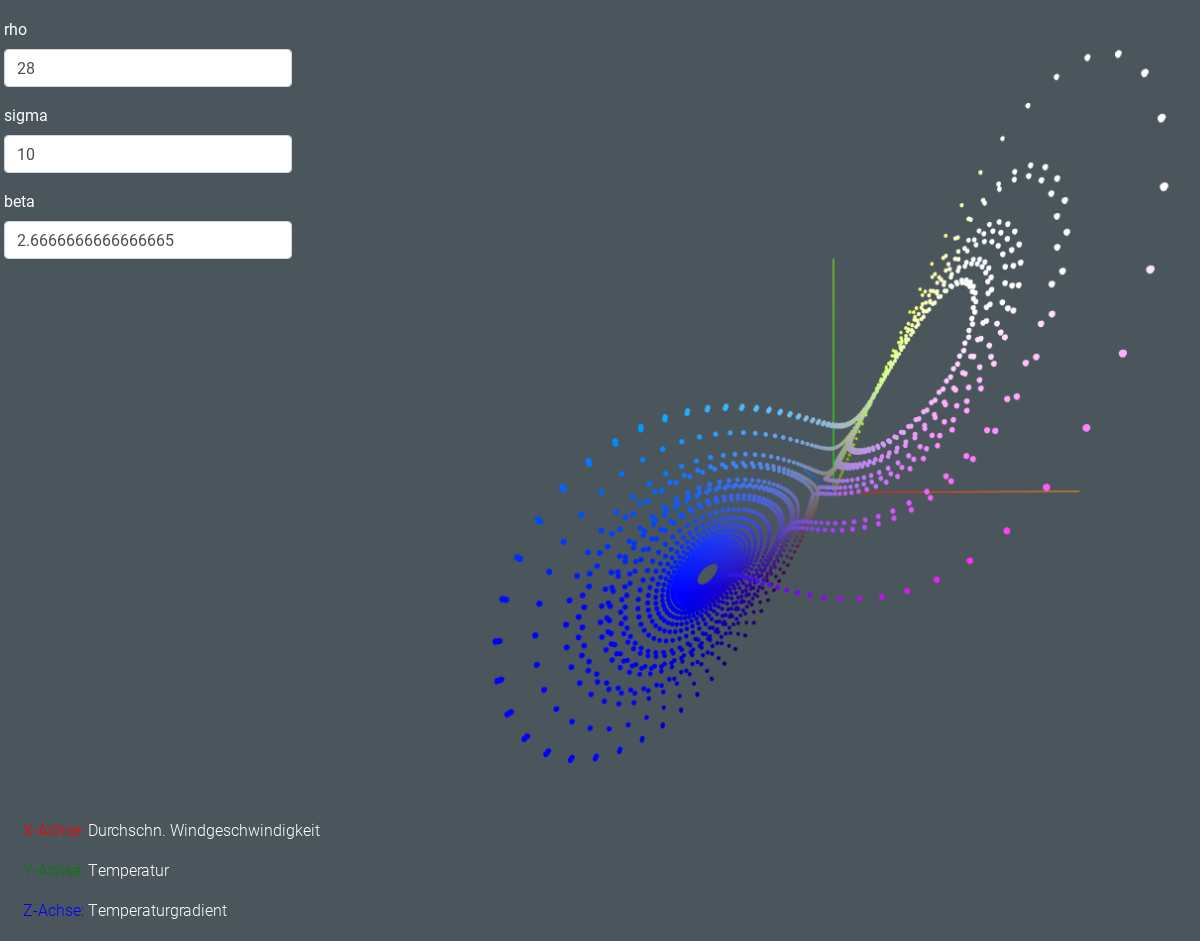
\includegraphics[height=5cm]{lorenz/assets/implementation/Visualisierung}
	\caption{Visualisierung Lorenz-Attraktor}
	\label{fig:visualisierung}
\end{figure}
